\documentclass[UTF8]{ctexart}
\usepackage{geometry}
\geometry{a4paper, margin=2.5cm}
\usepackage{graphicx}
\usepackage{listings}
\usepackage{xcolor}
\usepackage{float}
\usepackage{hyperref}
\usepackage{amsmath}
\usepackage{amssymb}
\usepackage{bm}
\usepackage{caption}
\usepackage{tikz}
\usetikzlibrary{arrows.meta}
\hypersetup{colorlinks=true, linkcolor=blue, urlcolor=blue}
\graphicspath{{D:/Repository/code/LATEX/Conmmunication/ChannelCoding/}}

\lstset{
    basicstyle=\ttfamily\small,
    breaklines=true,
    frame=single,
    numbers=left,
    numberstyle=\tiny,
    tabsize=4,
    language=MATLAB,
    keywordstyle=\color{blue},
    commentstyle=\color{green!60!black},
    stringstyle=\color{red}
}

\title{\textbf{信道编码与数字调制级联系统实验}}
\author{}

\begin{document}
\maketitle

\begin{center}
    \textbf{班级：}2024217802\quad \textbf{姓名：} 严子竣\quad \textbf{学号：}2024212622
\end{center}

\section{实验目的}
\begin{enumerate}
    \item 掌握卷积码的编码原理与 Viterbi 硬判决译码算法。
    \item 理解信道编码与数字调制级联系统的收发结构。
    \item 在 AWGN 信道下仿真 (2,1,3) 卷积码与 16‑QAM 的级联系统，对比未编码与编码后的误比特率（BER）和误帧率（BLER）。
    \item 观察卷积码带来的编码增益，分析纠错编码对系统性能的提升作用。
\end{enumerate}

\section{实验原理}

\subsection{(2,1,3) 卷积码}
卷积码是一种有记忆的纠错编码，编码器的输出不仅取决于当前输入比特，还与之前若干比特有关。本实验采用的卷积码参数为 (2,1,3)，即：
\begin{itemize}
    \item 码率 \(R_c = 1/2\)：每输入 1 个信息比特，输出 2 个编码比特。
    \item 约束长度 \(L = 3\)：编码器包含 2 个移位寄存器，状态数为 \(2^{L-1}=4\)。
    \item 生成多项式：\(g_1 = 7\)（二进制 111），\(g_2 = 5\)（二进制 101）。
\end{itemize}

设时刻 \(i\) 的输入比特为 \(u_i\)，移位寄存器状态为 \([s_{i-1}, s_{i-2}]\)，则两个输出比特为：
\begin{align}
    c_{i,1} &= u_i \oplus s_{i-1} \oplus s_{i-2} \\
    c_{i,2} &= u_i \oplus s_{i-2}
\end{align}
其中 \(\oplus\) 表示模 2 加法。

\subsection{Viterbi 硬判决译码}
Viterbi 算法是一种最大似然序列估计（MLSE）译码方法，通过动态规划在网格图上寻找与接收序列最匹配的路径。硬判决译码的步骤包括：
\begin{enumerate}
    \item 将接收到的编码比特进行 0/1 硬判决。
    \item 计算每步的分支度量（汉明距离）。
    \item 对每个状态，保留累计度量最小的路径。
    \item 通过回溯得到译码输出序列。
\end{enumerate}
本实验中，每帧信息比特后添加 2 个“0”尾比特，强制编码器回到全零状态，从而简化回溯。

\subsection{级联系统模型}
整个通信链路如图 \ref{fig:system_tikz} 所示。

\begin{figure}[H]
    \centering
    \begin{tikzpicture}[>=stealth, node distance=1.2cm, auto, 
        block/.style={rectangle, draw, minimum width=1.8cm, minimum height=0.8cm, align=center, font=\small},
        sum/.style={circle, draw, minimum size=0.6cm, inner sep=0pt}]
        
        % 节点
        \node (source) {信源};
        \node[block, right of=source, node distance=2.2cm] (encoder) {卷积码\\编码器};
        \node[block, right of=encoder, node distance=2.5cm] (mod) {16‑QAM\\调制器};
        \node[sum, right of=mod, node distance=2.2cm] (add) {$+$};
        \node[below of=add, node distance=1cm] (noise) {高斯噪声};
        \node[block, right of=add, node distance=2.2cm] (demod) {16‑QAM\\硬判决解调};
        \node[block, right of=demod, node distance=2.5cm] (decoder) {Viterbi\\硬译码};
        \node[right of=decoder, node distance=2.2cm] (sink) {信宿};
        
        % 连线
        \draw[->] (source) -- (encoder);
        \draw[->] (encoder) -- (mod);
        \draw[->] (mod) -- (add);
        \draw[->] (noise) -- (add);
        \draw[->] (add) -- (demod);
        \draw[->] (demod) -- (decoder);
        \draw[->] (decoder) -- (sink);
        
        % 添加标注文字
        \node[above] at (encoder.north) {信息比特};
        \node[above] at (mod.north) {编码符号};
        \node[above] at (demod.north) {接收符号};
        \node[above] at (decoder.north) {硬判决比特};
        
        % 信道标注
        \node at (add.south east)[above,yshift=0.5cm]{AWGN 信道};
    \end{tikzpicture}
    \caption{编码调制级联系统框图}
    \label{fig:system_tikz}
\end{figure}

\subsection{性能指标}
\begin{itemize}
    \item \textbf{BER}：误比特率，错误比特数占总传输比特数的比例（仅统计信息比特）。
    \item \textbf{BLER}：误帧率，错误帧数占总传输帧数的比例。一帧内只要有一个信息比特错误即判为帧错误。
\end{itemize}
编码增益定义为在相同 BER 下，编码系统所需的 \(E_b/N_0\) 相比于未编码系统的降低量。

\section{仿真参数设置}
本次仿真的参数如表 \ref{tab:params} 所示。

\begin{table}[H]
    \centering
    \caption{仿真参数配置}
    \begin{tabular}{|c|c|}
        \hline
        \textbf{参数} & \textbf{数值} \\
        \hline
        调制阶数 \(M\) & 16 \\
        \hline
        每符号比特数 \(k\) & 4 \\
        \hline
        每帧符号数 \(N_{\text{sym}}\) & 10000 \\
        \hline
        每帧比特数（编码后） & 40000 \\
        \hline
        每帧信息比特数 & \(40000/2 - 2 = 19998\) \\
        \hline
        尾比特数 & 2 \\
        \hline
        仿真帧数（每信噪比点） & 100 \\
        \hline
        信噪比范围 \(E_b/N_0\) (dB) & 0, 2, 4, 6, 8, 10, 12, 14 \\
        \hline
        卷积码 & (2,1,3), 生成多项式 [7,5] \\
        \hline
        译码方式 & Viterbi 硬判决 \\
        \hline
    \end{tabular}
    \label{tab:params}
\end{table}

\section{仿真结果与分析}

运行 MATLAB 代码 \texttt{ChannelCoding.m} 得到图 \ref{fig:result} 所示的性能曲线。

\begin{figure}[H]
    \centering
    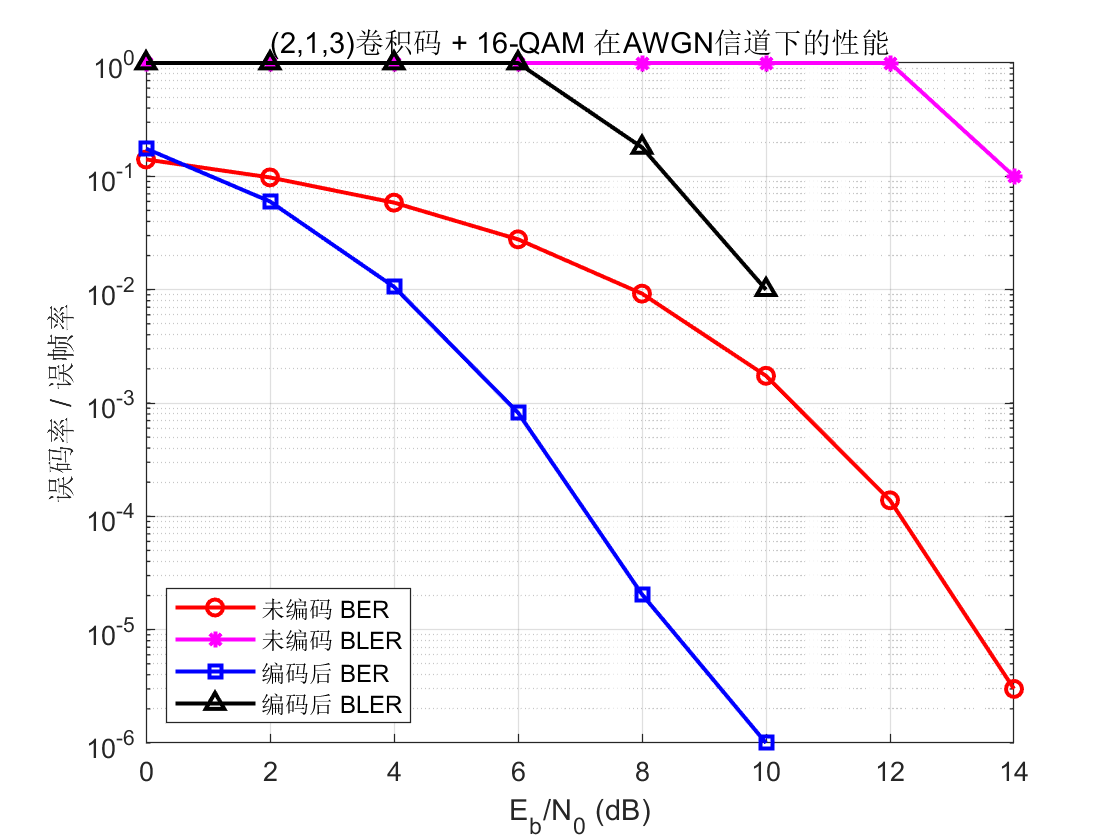
\includegraphics[width=0.8\textwidth]{channelcoding.png}
    \caption{未编码与 (2,1,3) 卷积码 + 16‑QAM 级联系统的 BER/BLER 性能对比}
    \label{fig:result}
\end{figure}

\subsection{误比特率（BER）分析}
从图 \ref{fig:result} 中可以看出：
\begin{itemize}
    \item 在低信噪比区域（\(E_b/N_0 \leq 2\) dB），编码系统的 BER 甚至略高于未编码系统。这是因为译码器在极低信噪比下可能产生错误传播，且硬判决丢失了可靠性信息。
    \item 当 \(E_b/N_0 \geq 4\) dB 时，编码增益开始显现，编码系统的 BER 下降速度明显快于未编码系统，体现了卷积码的纠错能力。
    \item 在高信噪比区域（\(E_b/N_0 \geq 10\) dB），编码系统的 BER 过低，由于一帧仅有$k\cdot N_{\text{sym}}=40000$bit，低于$10^{-6}$的BER无法在图中显示。本次仿真中，\(E_b/N_0 = 10\) dB恰好有一帧中的一个比特发生错误，因此观测到$10^{-6}$的BER
\end{itemize}

\subsection{误帧率（BLER）分析}
\begin{itemize}
    \item 编码系统的 BLER 曲线与 BER 曲线形状相似，但数值更高。这是因为每帧包含近 20000 个信息比特，只要有一个未被纠正的比特错误就会导致帧错误。
    \item 编码系统在 BLER 方面同样获得显著增益，例如在 \(\text{BLER}=10^{-1}\) 处增益约为 5.5 dB。
\end{itemize}

\section{实验总结}
\begin{enumerate}
    \item 实现了 (2,1,3) 卷积码的编码器和 Viterbi 硬判决译码器。
    \item 通过仿真对比了未编码与编码系统的 BER/BLER 性能，验证了卷积码在中高信噪比下的明显增益。
    \item 硬判决译码在低信噪比区域存在性能损失，但整体仍能提供 4～5 dB 的编码增益。
\end{enumerate}

\end{document}